\documentclass[tikz,border=5pt]{standalone}

\usetikzlibrary{calc, intersections}
\usepackage{xfp}

\begin{document}
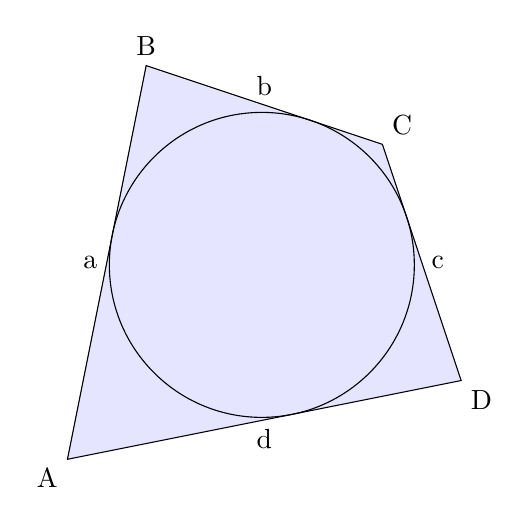
\begin{tikzpicture}

% Define Coordinates of the quadrilateral

% This quadrilateral have incenter
\coordinate (A) at (0,0);
\coordinate (B) at (1,5);
\coordinate (C) at (4,4);
\coordinate (D) at (5,1);

% This quadrilateral doesn't have incenter.
%% \coordinate (A) at (0,0);
%% \coordinate (B) at (5,1);
%% \coordinate (C) at (4,1);
%% \coordinate (D) at (1,5);

% Calcular longitud de los lados
\path let \p1=(A), \p2=(B), \p3=(C), \p4=(D)
    in node[draw=none] at (0,0) {
        \xdef\sideAB{\fpeval{sqrt((\x2-\x1)^2 + (\y2-\y1)^2)}}
        \xdef\sideBC{\fpeval{sqrt((\x3-\x2)^2 + (\y3-\y2)^2)}}
        \xdef\sideCD{\fpeval{sqrt((\x4-\x3)^2 + (\y4-\y3)^2)}}
        \xdef\sideDA{\fpeval{sqrt((\x1-\x4)^2 + (\y1-\y4)^2)}}
    };

% Logical Check (Precision up to 0.001)
%
% The 'e' in \edef stands for expanded. It tells TE​X: "Read everything inside the curly braces right now, replace all variables with their current values, and store the final result."
\edef\isTangential{\fpeval{abs(\fpeval{\sideAB + \sideCD} - \fpeval{\sideBC + \sideDA}) < 0.001 ? 1 : 0}}

\ifnum\isTangential=1

    % Dibujar cuadrilátero y sus vértices

    \draw[fill=blue!10!white]
             (A) node[below left]{A}
          -- node[left]{a} (B) node[above]{B}
          -- node[above]{b} (C) node[above right]{C}
          -- node[right]{c} (D) node[below right]{D}
          -- node[below]{d} cycle;

    %% Dibujar circunferencia inscrita al cuadrilátero

    % Angle bisector 1
    \coordinate(G1) at ($(A)!1cm!(B)$); % Coordinate located at 1 cm from A towards B
    \coordinate(G2) at ($(A)!1cm!(D)$); % Coordinate located at 1 cm from A towards D
    \coordinate(M1) at ($(G1)!.5!(G2)$); % Midpoint between G1 and G2
    \path[name path=bisc1]
        let \p1=(A), \p2=(C), \n1={veclen(\y2-\y1,\x2-\x1)} % Calculate distance between A and C
        in (A) -- ($(A)!\n1!(M1)$); % Draw a segment from A towards M1 with length equal to the distance AC

    % Angle bisector 2
    \coordinate(H1) at ($(B)!1cm!(A)$);
    \coordinate(H2) at ($(B)!1cm!(C)$);
    \coordinate(M2) at ($(H1)!.5!(H2)$);
    \path[name path=bisc2]
        let \p1=(B), \p2=(D), \n1={veclen(\y2-\y1,\x2-\x1)} % Calculate distance between B and D
        in (B) -- ($(B)!\n1!(M2)$); % Draw a segment from B towards M2 with length equal to the distance BD

    \draw [name intersections={of=bisc1 and bisc2, by={centerOfIncircle}}]
        % The syntax (P_1)!(P_2)!(P_3) tells TikZ to find the point on the line segment \bar{P_1P_3} that is closest to P_2.
        % Here, p2 is the orthogonal projection of the center onto the segment AB. In other words, \bar{p1p2} is a radius.
        % n1 is the length of the radius
        let \p1=(centerOfIncircle), \p2=($(A)!(centerOfIncircle)!(B)$), \n1={veclen(\y2-\y1,\x2-\x1)}
        in (centerOfIncircle) circle [radius=\n1];
\else
    % Display the warning message
    \node[red, font=\bfseries] at (0,0) {This quadrilateral doesn't have an incircle. $\sumOne \approx \sumTwo$};
\fi
\end{tikzpicture}
\end{document}
